\documentclass{beamer}
% imprimir
% \documentclass[handout]{beamer} 
% \usepackage{pgfpages}
% \pgfpagesuselayout{4 on 1}[a4paper,landscape,border shrink=5mm]

\mode<presentation> {
  \usetheme{Warsaw}
  \setbeamercovered{transparent}
}

\usebackgroundtemplate{
\includegraphics[width=\paperwidth]{format/libresoft-bg.png}}
\usepackage[spanish]{babel}
\usepackage[utf8]{inputenc}
\usepackage{graphics}
\usepackage{amssymb} % Simbolos matematicos

%\definecolor{libresoftgreen}{RGB}{162,190,43}
%\definecolor{libresoftblue}{RGB}{0,98,143}

%\setbeamercolor{titlelike}{bg=libresoftgreen}

%% Metadatos del PDF.
\hypersetup{  
  pdftitle={El software libre en el lado del servidor},
  pdfauthor={Miguel Vidal},
  pdfcreator={GSyC/Libresoft},
  pdfproducer=PDFLaTeX,
  pdfsubject={Master on Libre Software},
}
%%

\begin{document}

\title{El software libre en el lado del servidor}
\subtitle{Master on Libre Software}
\institute{\{mvidal,jfcastro\}@libresoft.es} 
\author{Miguel Vidal, José Castro}
\date{\today}

\frame{
\maketitle
\begin{center}

\includegraphics[width=6cm]{format/gsyc-urjc}
\end{center}
}

%% License slide
\begin{frame}
  \vspace{2cm}
  \begin{flushright}
    {\footnotesize \copyright{} 2009-2011 Miguel Vidal, Jose Castro.} \\
%    \vspace{0.25cm}
    \medskip
    {\scriptsize Esta presentación se distribuye bajo \\ licencia Creative Commons Reconocimiento 3.0 España}
%    \vspace{0.10cm}
  \end{flushright}
  \begin{center}
    \href{http://creativecommons.org/licenses/by/3.0/es}{
\includegraphics[width=2cm]{format/cc-by.png}} \\
    {\tiny \url{http://creativecommons.org/licenses/by/3.0/es}}
  \end{center}
\end{frame}%%

%%%%%%%%%%%%%%%%%%%%%%%%%%%%%%%%%%%%%%%%%%%%%%%%%%%%%%%%%%%%%%%%%%%%%%%

\begin{frame}
\frametitle{¿Quiénes somos?}

\begin{itemize}
\item \alert{Miguel Vidal} (\url{http://gsyc.es/~mvidal}): 


	\begin{itemize}

\footnotesize

	\item Desplegó la actual infraestructura HA de \href{http://www.morfeo-project.org}{Morfeo} y ha colaborado en la administración y mantenimiento a bajo nivel de la plataforma \href{http://www.osor.eu}{OSO-R}. 
	\item Administró los servidores de barrapunto.com durante seis años.
	\item Responsable del proyecto de traducción al español de la \href{http://www.openbsd.org/translation.html\#WHO}{documentación de OpenBSD}.
	\end{itemize}

\normalsize

\item \alert{José Castro} (\url{http://gsyc.es/~jfcastro}): 

	\begin{itemize}

\footnotesize

	\item Responsable de sistemas de la plataforma HA de \href{http://www.morfeo-project.org}{Morfeo}. 
	\item Parte del equipo técnico de la plataforma europea \href{http://www.osor.eu}{OSO-R}.
	\item Miembro fundador de Madrid-OSUG (comunidad de usuarios de OpenSolaris en Madrid).
	\end{itemize}

\end{itemize}
\end{frame}

\normalsize


%%%%%%%%%%%%%%%%%%%%%%%%%%%%%%%%%%%%%%%%%%%%%%%%%%%%%%%%%%%%%%%%%%%%%%%
\section{Software libre en servidores}
%%%%%%%%%%%%%%%%%%%%%%%%%%%%%%%%%%%%%%%%%%%%%%%%%%%%%%%%%%%%%%%%%%%%%%%

\begin{frame}

\begin{center}
\huge{Software libre en servidores}
\end{center}

\end{frame}



%%%%%%%%%%%%%%%%%%%%%%%%%%%%%%%%%%%%%%%%%%%%%%%%%%%%%%%%%%%%%%%%%%%%%%%

\begin{frame}
\frametitle{Ventajas del software libre en servidores (I)}

\begin{itemize}
\item Libertad de uso, modificación y redistribución: 
	\begin{itemize}
	\item podemos \alert{instalarlo} en tantas máquinas como queramos.
	\item podemos \alert{adaptarlo} a nuestras necesidades o las del cliente.
	\item podemos revisar el código y \alert{corregir} errores sin esperar a que lo haga el fabricante.
	\item podemos beneficiarnos de las mejoras y correcciones que hagan otros.
	\end{itemize}

\item  Corrección mas rápida y eficiente de fallos, y rápida resolución de dudas y problemas, gracias al \alert{modelo bazar} y a las fuertes comunidades que tiene detrás.

\end{itemize}
\end{frame}

%%%%%%%%%%%%%%%%%%%%%%%%%%%%%%%%%%%%%%%%%%%%%%%%%%%%%%%%%%%%%%%%%%%%%%%

\begin{frame}
\frametitle{Ventajas del software libre en servidores (II)}

\begin{itemize}
\item \alert{Independencia tecnológica}: no nos atamos a ningún proveedor en particular.
\item Soporte y \alert{compatibilidad} a largo plazo: el fabricante no está forzado a ``vendernos'' continuamente nuevas versiones. 
\item Fomento de la \alert{libre competencia} al basarse en servicios y no en licencias.
\item Ausencia de secretismo tecnológico y de patentes (seguridad jurídica). 
\item \alert{Formatos estándar}: facilitan la interoperabilidad y evitan incompatibilidades. 
\item Métodos simples y unificados de gestión de software: las distribuciones evitan tener que acudir a buscar software de fuentes dudosas.
\end{itemize}
\end{frame}

%%%%%%%%%%%%%%%%%%%%%%%%%%%%%%%%%%%%%%%%%%%%%%%%%%%%%%%%%%%%%%%%%%%%%%%

\begin{frame}
\frametitle{Ventajas del software libre en servidores (y III)}

\begin{itemize}
\item Inmensa \alert{variedad} de soluciones muy \alert{maduras}: el software libre nace en entornos de servidores.
\item Demanda de técnicos FLOSS en expansión, gracias a la creciente adopción por parte de las AA.PP. y de grandes empresas tecnológicas (Google, IBM, Sun/Oracle, etc.).
\item Sistemas \alert{potencialmente más seguros}: hackers y empresas de seguridad de todo el mundo puedan auditar los programas.
\item Aspectos económicos: más de mil millones de euros en licencias de Microsoft en España anuales (2006). Bajo TCO.
\item Fiabilidad y rendimiento.
\end{itemize}
\end{frame}

%%%%%%%%%%%%%%%%%%%%%%%%%%%%%%%%%%%%%%%%%%%%%%%%%%%%%%%%%%%%%%%%%%%%%%%

\begin{frame}
\frametitle{Mercado de servidores con software libre}

\begin{itemize}
\item El mercado suele medirse por unidades vendidas o por beneficios
\item Difícil de evaluar para el caso del FLOSS: sistemas libres son a menudo obtenidos sin coste e instalados sin contratar soporte.
\item Muchas veces se instalan en máquinas que no fueron compradas con software libre precargado.
\item El método que se usa suele ser mediante acceso a máquinas públicamente accesibles (como servidores web).
\item Problema: este método no contempla las máquinas no accesibles públicamente.
\end{itemize}
\end{frame}


%%%%%%%%%%%%%%%%%%%%%%%%%%%%%%%%%%%%%%%%%%%%%%%%%%%%%%%%%%%%%%%%%%%%%%%

\begin{frame}
\frametitle{Mercado de servidores}

\begin{center}
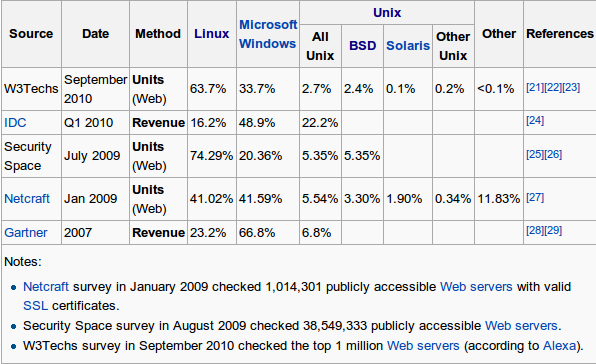
\includegraphics[width=11.0cm]{figs/servers-market.png}
\end{center}

\end{frame}

%%%%%%%%%%%%%%%%%%%%%%%%%%%%%%%%%%%%%%%%%%%%%%%%%%%%%%%%%%%%%%%%%%%%%%%

\begin{frame}
\frametitle{Compañías de hosting más fiables}

\begin{center}
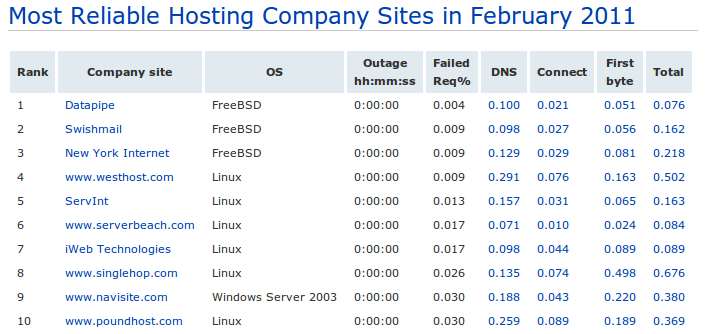
\includegraphics[width=11.5cm]{figs/netcraft.png}
\end{center}

\end{frame}

%%%%%%%%%%%%%%%%%%%%%%%%%%%%%%%%%%%%%%%%%%%%%%%%%%%%%%%%%%%%%%%%%%%%%%%

\begin{frame}
\frametitle{¿No hay desventajas?}
\setbeamercovered{invisible}

\pause

\begin{itemize}
\item Necesidad de técnicos especializados (la gente se forma con SO privativos)
\item Interfaces visuales (suelen ser privativos)
\item No siempre hay soporte para todo tipo de hardware (patentes, drivers y especificaciones privativas).
\item Suele ser necesario hacer \textit{advocacy} y plantear migraciones.
\item ¿Mayor mercado laboral en sistemas privativos? (depende del sector)
\end{itemize}
\end{frame}

%%%%%%%%%%%%%%%%%%%%%%%%%%%%%%%%%%%%%%%%%%%%%%%%%%%%%%%%%%%%%%%%%%%%%%%

\begin{frame}
\frametitle{¿Y qué hay de las GUIs?}


\setbeamercovered{invisible}

\pause

\begin{itemize}
\item Muchas distros traen GUIs o herramientas visuales propias. 
\item Son útiles y facilitan las tareas, sobre todo para sysadmins noveles.

\pause

	\begin{itemize}
	\item Suelen ser privativas
	\item O nos hacen dependientes de una distro en concreto
	\item A veces poseen oscuros detalles en la forma de gestionar los recursos
	\end{itemize}

\pause

\item Las tecnologías y métodos subyacentes suelen ser comunes a todas las distros, incluso a todos los Unixes.

\pause

\item La configuración manual es mejor: más rápida, más flexible, más fiable, más potente y más \textit{scriptable}.
\end{itemize}
\end{frame}



%%%%%%%%%%%%%%%%%%%%%%%%%%%%%%%%%%%%%%%%%%%%%%%%%%%%%%%%%%%%%%%%%%%%%%%

\begin{frame}
\frametitle{¿Es gratis el software libre? Algunos consejos}

\pause

\begin{itemize}
\item La gratuidad no es el punto fuerte del software libre
\item Insistir en la gratuidad supone minusvalorar el resto de ventajas (y es injusto para la gente que lo crea y lo mantiene).
\item No comiences hablándoles de dinero a los que toman decisiones. 
\item No hablar del FLOSS en abstracto (``Linux es mejor''): estudia costes de migración y trata de cubrir necesidades concretas que no están cubiertas o mejorar lo que hay.
\item No seas impaciente: deja que el software libre crezca con los clientes, introduciendo mejoras de forma progresiva.
\end{itemize}
\end{frame}


%%%%%%%%%%%%%%%%%%%%%%%%%%%%%%%%%%%%%%%%%%%%%%%%%%%%%%%%%%%%%%%%%%%%%%%

\begin{frame}
\frametitle{Unix Culture}

\begin{itemize}
\item ``KISS'', ``Small is beautiful'', ``Make each program do one thing well'', ``Build a prototype as soon as possible'', ``Choose portability over efficiency'', ``Use shell scripts to increase leverage and portability'', ``Avoid captive user interfaces'', ``Make every program a filter''...
\item ``Worse is better'': design style and simplicity is more important than correctness, consistency and completeness.
\item Usenet, Internet jargon... 
\item System Administrator Appreciation Day (last Friday in July)
\item Bastard Operator From Hell (BOFH)
\end{itemize}
\end{frame}


\end{document}




